% OLD
%\documentclass[11pt,compress,t,notes=noshow, aspectratio=169, xcolor=table]{beamer}
% new
\\documentclass[10pt,compress,t,notes=noshow, xcolor=table]{beamer}

% OLD
%\usepackage{../../style/lmu-lecture}
% new
% graphicx and color are loaded via lmu-lecture.sty
% maxwidth is the original width if it is less than linewidth
% otherwise use linewidth (to make sure the graphics do not exceed the margin)
% TODO: Remove once cleared to be superfluous
% \makeatletter
% \def\maxwidth{ %
%   \ifdim\Gin@nat@width>\linewidth
%     \linewidth
%   \else
%     \Gin@nat@width
%   \fi
% }
% \makeatother

% ---------------------------------%
% latex-math dependencies, do not remove:
% - mathtools
% - bm
% - siunitx
% - dsfont
% - xspace
% ---------------------------------%

%--------------------------------------------------------%
%       Language, encoding, typography
%--------------------------------------------------------%

\usepackage[english]{babel}
\usepackage[utf8]{inputenc} % Enables inputting UTF-8 symbols
% Standard AMS suite (loaded via lmu-lecture.sty)

% Font for double-stroke / blackboard letters for sets of numbers (N, R, ...)
% Distribution name is "doublestroke"
% According to https://mirror.physik.tu-berlin.de/pub/CTAN/fonts/doublestroke/dsdoc.pdf
% the "bbm" package does a similar thing and may be superfluous.
% Required for latex-math
\usepackage{dsfont}

% bbm – "Blackboard-style" cm fonts (https://www.ctan.org/pkg/bbm)
% Used to be in common.tex, loaded directly after this file
% Maybe superfluous given dsfont is loaded
% TODO: Check if really unused?
% \usepackage{bbm}

% bm – Access bold symbols in maths mode - https://ctan.org/pkg/bm
% Required for latex-math, preferred over \boldsymbol
% https://tex.stackexchange.com/questions/3238/bm-package-versus-boldsymbol
\usepackage{bm}

% pifont – Access to PostScript standard Symbol and Dingbats fonts
% Used for \newcommand{\xmark}{\ding{55}, which is never used
% aside from lecture_advml/attic/xx-automl/slides.Rnw
% \usepackage{pifont}

% Quotes (inline and display), provdes \enquote
% https://ctan.org/pkg/csquotes
\usepackage{csquotes}

% Adds arg to enumerate env, technically superseded by enumitem according
% to https://ctan.org/pkg/enumerate
% Replace with https://ctan.org/pkg/enumitem ?
% Even better: enumitem is not really compatible with beamer and breaks all sorts of things
% particularly the enumerate environment. The enumerate package also just isn't required
% from what I can tell so... don't re-add it I guess?
% \usepackage{enumerate}

% Line spacing - provides \singlespacing \doublespacing \onehalfspacing
% https://ctan.org/pkg/setspace
% \usepackage{setspace}

% mathtools – Mathematical tools to use with amsmath
% https://ctan.org/pkg/mathtools?lang=en
% latex-math dependency according to latex-math repo
\usepackage{mathtools}

% Maybe not great to use this https://tex.stackexchange.com/a/197/19093
% Use align instead -- TODO: Global search & replace to check, eqnarray is used a lot
% $ rg -f -u "\begin{eqnarray" -l | grep -v attic | awk -F '/' '{print $1}' | sort | uniq -c
%   13 lecture_advml
%   14 lecture_i2ml
%    2 lecture_iml
%   27 lecture_optimization
%   45 lecture_sl
\usepackage{eqnarray}
% For shaded regions / boxes
% Used sometimes in optim
% https://www.ctan.org/pkg/framed
\usepackage{framed}

%--------------------------------------------------------%
%       Cite button (version 2024-05)
%--------------------------------------------------------%

% Superseded by style/ref-buttons.sty, kept just in case these don't work out somehow.

% Note this requires biber to be in $PATH when running,
% telltale error in log would be e.g. Package biblatex Info: ... file 'authoryear.dbx' not found
% aside from obvious "biber: command not found" or similar.
% Tried moving this to lmu-lecture.sty but had issues I didn't quite understood,
% so it's here for now.

\usepackage{hyperref}

% Only try adding a references file if it exists, otherwise
% this would compile error when references.bib is not found
% NOTE: Bibliography packages (usebib, biblatex) are now loaded by ref-buttons.sty when needed
% This keeps all bibliography-related setup in one place

% Legacy \citelink command removed - superseded by ref-buttons.sty

%--------------------------------------------------------%
%       Displaying code and algorithms
%--------------------------------------------------------%

% Reimplements verbatim environments: https://ctan.org/pkg/verbatim
% verbatim used sed at least once in
% supervised-classification/slides-classification-tasks.tex
% Removed since code should not be put on slides anyway
% \usepackage{verbatim}

% Both used together for algorithm typesetting, see also overleaf: https://www.overleaf.com/learn/latex/Algorithms
% algorithmic env is also used, but part of the bundle:
%   "algpseudocode is part of the algorithmicx bundle, it gives you an improved version of algorithmic besides providing some other features"
% According to https://tex.stackexchange.com/questions/229355/algorithm-algorithmic-algorithmicx-algorithm2e-algpseudocode-confused
\usepackage{algorithm}
\usepackage{algpseudocode}

%--------------------------------------------------------%
%       Tables
%--------------------------------------------------------%

% multi-row table cells: https://www.namsu.de/Extra/pakete/Multirow.html
% Provides \multirow
% Used e.g. in evaluation/slides-evaluation-measures-classification.tex
\usepackage{multirow}

% colortbl: https://ctan.org/pkg/colortbl
% "The package allows rows and columns to be coloured, and even individual cells." well.
% Provides \columncolor and \rowcolor
% \rowcolor is used multiple times, e.g. in knn/slides-knn.tex
\usepackage{colortbl}

% long/multi-page tables: https://texdoc.org/serve/longtable.pdf/0
% Not used in slides
% \usepackage{longtable}

% pretty table env: https://ctan.org/pkg/booktabs
% Is used
% Defines \toprule
\usepackage{booktabs}

%--------------------------------------------------------%
%       Figures: Creating, placing, verbing
%--------------------------------------------------------%

% wrapfig - Wrapping text around figures https://de.overleaf.com/learn/latex/Wrapping_text_around_figures
% Provides wrapfigure environment -used in lecture_optimization
\usepackage{wrapfig}

% Sub figures in figures and tables
% https://ctan.org/pkg/subfig -- supersedes subfigure package
% Provides \subfigure
% \subfigure not used in slides but slides-tuning-practical.pdf errors without this pkg, error due to \captionsetup undefined
\usepackage{subfig}

% Actually it's pronounced PGF https://en.wikibooks.org/wiki/LaTeX/PGF/TikZ
\usepackage{tikz}

% No idea what/why these settings are what they are but I assume they're there on purpose
\usetikzlibrary{shapes,arrows,automata,positioning,calc,chains,trees, shadows}
\tikzset{
  %Define standard arrow tip
  >=stealth',
  %Define style for boxes
  punkt/.style={
    rectangle,
    rounded corners,
    draw=black, very thick,
    text width=6.5em,
    minimum height=2em,
    text centered},
  % Define arrow style
  pil/.style={
    ->,
    thick,
    shorten <=2pt,
    shorten >=2pt,}
}

%--------------------------------------------------------%
%       Beamer setup and custom macros & environments
%--------------------------------------------------------%

% Main sty file for beamer setup (layout, style, lecture page numbering, etc.)
% For long-term maintenance, this may me refactored into a more modular set of .sty files
\usepackage{../../style/lmu-lecture}
% Custom itemize wrappers, itemizeS, itemizeL, etc
\usepackage{../../style/customitemize}
% Custom framei environment, uses custom itemize!
\usepackage{../../style/framei}
% Custom frame2 environment, allows specifying font size for all content
\usepackage{../../style/frame2}
% Column layout macros
\usepackage{../../style/splitV}
% \image and derivatives
\usepackage{../../style/image}
% New generation of reference button macros
\usepackage{../../style/ref-buttons}

% Used regularly
\let\code=\texttt

% Not sure what/why this does
\setkeys{Gin}{width=0.9\textwidth}

% -- knitr leftovers --
% These may be used by knitr/R Markdown workflows in other lectures
\makeatletter
\def\maxwidth{ %
  \ifdim\Gin@nat@width>\linewidth
    \linewidth
  \else
    \Gin@nat@width
  \fi
}
\makeatother

% Define colors for syntax highlighting (may be used by knitr)
\definecolor{fgcolor}{rgb}{0.345, 0.345, 0.345}
\definecolor{shadecolor}{rgb}{.97, .97, .97}

% knitr code output environment
\newenvironment{knitrout}{}{}


% Can't find a reason why common.tex is not just part of this file?
% This file is included in slides and exercises

% Rarely used fontstyle for R packages, used only in 
% - forests/slides-forests-benchmark.tex
% - exercises/single-exercises/methods_l_1.Rnw
% - slides/cart/attic/slides_extra_trees.Rnw
\newcommand{\pkg}[1]{{\fontseries{b}\selectfont #1}}

% Spacing helpers, used often (mostly in exercises for \dlz)
\newcommand{\lz}{\vspace{0.5cm}} % vertical space (used often in slides)
\newcommand{\dlz}{\vspace{1cm}}  % double vertical space (used often in exercises, never in slides)
\newcommand{\oneliner}[1] % Oneliner for important statements, used e.g. in iml, algods
{\begin{block}{}\begin{center}\begin{Large}#1\end{Large}\end{center}\end{block}}

% Don't know if this is used or needed, remove?
% textcolor that works in mathmode
% https://tex.stackexchange.com/a/261480
% Used e.g. in forests/slides-forests-bagging.tex
% [...] \textcolor{blue}{\tfrac{1}{M}\sum^M_{m} [...]
% \makeatletter
% \renewcommand*{\@textcolor}[3]{%
%   \protect\leavevmode
%   \begingroup
%     \color#1{#2}#3%
%   \endgroup
% }
% \makeatother


% Defines macros and environments
% This file is included in slides and exercises

% Rarely used fontstyle for R packages, used only in 
% - forests/slides-forests-benchmark.tex
% - exercises/single-exercises/methods_l_1.Rnw
% - slides/cart/attic/slides_extra_trees.Rnw
\newcommand{\pkg}[1]{{\fontseries{b}\selectfont #1}}

% Spacing helpers, used often (mostly in exercises for \dlz)
\newcommand{\lz}{\vspace{0.5cm}} % vertical space (used often in slides)
\newcommand{\dlz}{\vspace{1cm}}  % double vertical space (used often in exercises, never in slides)
\newcommand{\oneliner}[1] % Oneliner for important statements, used e.g. in iml, algods
{\begin{block}{}\begin{center}\begin{Large}#1\end{Large}\end{center}\end{block}}

% Don't know if this is used or needed, remove?
% textcolor that works in mathmode
% https://tex.stackexchange.com/a/261480
% Used e.g. in forests/slides-forests-bagging.tex
% [...] \textcolor{blue}{\tfrac{1}{M}\sum^M_{m} [...]
% \makeatletter
% \renewcommand*{\@textcolor}[3]{%
%   \protect\leavevmode
%   \begingroup
%     \color#1{#2}#3%
%   \endgroup
% }
% \makeatother

\newcommand{\open}{}
\newcommand{\close}{}

\title{Interpretable Machine Learning}
% \author{LMU}
%\institute{\href{https://compstat-lmu.github.io/lecture_iml/}{compstat-lmu.github.io/lecture\_iml}}
\date{}

\begin{document}

%Gliederung:
%- Intro with examples, motivation, problems
%- standard fANOVA calculation + example
%- from that intuition & motivation: h-statistic  ->  move that after theory ??
%- conditions + theory
%- other methods (gen fANOVA, ALE)

% OLD
%\newcommand{\titlefigure}{figure/25-05-31_Hooker_2004_graph_fANOVA}
%\newcommand{\learninggoals}{
%\item Basic idea of additive functional decompositions
%\item Motivation and usefulness of functional decompositions
%\item Difficulty of obtaining or even defining a functional decomposition
%\item Several examples
%}
%
%\lecturechapter{Introduction to Functional Decomposition}
%\lecture{Interpretable Machine Learning}
% new
\titlemeta{
Introduction to Functional Decomposition
}{
Interpretable Machine Learning
}{
figure/25-05-31_Hooker_2004_graph_fANOVA
}{

\item Basic idea of additive functional decompositions
\item Motivation and usefulness of functional decompositions
\item Difficulty of obtaining or even defining a functional decomposition
\item Several examples

}



\begin{frame}{Preliminaries}

    \textbf{Recap: Interactions}
    \begin{itemize}
        \item Interactions between features: Effect of one feature on the prediction output depends on (one or more) other features
        \item Definition: Features $x_j$  and $x_k$ are considered to interact, if
        $$
        \mathbb{E} \left[ \left( \frac{\partial^2 f(\xv)}{\partial x_j \partial x_k} \right)^2 \right] > 0
        $$
    \end{itemize}
    
    \pause
    \textbf{Recap: GAMs}
    \begin{itemize}
        \item Decomposition into only main effects
        \item Do not contain any interactions
    \end{itemize}
    $$
    \fh (\xv) = \theta_0 + g_1(x_1) + g_2(x_2) + \ldots + g_p(x_p)
    $$
    % Recap: Interactions between features: The effect of some features on the prediction output depends on (one or more) other features \\
    % This cannot be captured by the main feature effects alone (i.e. by a GAM).
    % We want to know, which parts are attributed to effects of single features (s.o. feature effect methods), and which to interactions.

    % Idea throughout the whole chapter: GAMs have decomposition into main effects and don't contain any interactions

    % \textit{
    % TO DO: After introducing PDPs and PD-functions more generally in chapter 3, we would want to introduce H-statistic as a measure / as a possible definition for interactions, maybe even in the general case (i.e. the H-statistic for testing for an \(n\)-way interaction between \(n\) many features). \\
    % First introduce the more general concept of \(k\)-way interactions between any \(k\) groups of variables. \\
    % Remember EBMs at this point: There, strong interactions were defined via reduction in RSS compared to a univariate model / a GAM -> exactly same idea / same formula
    % }

\end{frame}

\begin{frame}{First Example: Additive decomposition}

    \begin{example}

    Consider
    $$
    \fh(x_1, x_2) = 4 - 2x_1 + 0.3 e^{x_2} + |x_1|x_2
    $$
    % The function \( \fh(x_1, x_2) = 4 - 2x_1 + 0.3 e^{x_2} + |x_1|x_2 \) depends on two features, and contains the interaction \( |x_1|x_2 \) between the two features.

    \begin{itemize}
    
        \item Idea: Additive decomposition depending on which features used:
        
        \pause
        \begin{equation}\label{eq:func_decomp_first_min_example}
        \begin{aligned}
            & g_\emptyset(x_1, x_2) = 4 & \text{ Part depending on no features at all (intercept)}  \\
            &
            \left.\begin{aligned}
                & g_1(x_1, x_2) = 2x_1 \\
                & g_2(x_1, x_2) = 0.3 e^{x_2}
            \end{aligned}\right\}
                & \text{ Parts depending on a single feature (main effects)}  \\
            & g_{1,2}(x_1, x_2) = |x_1|x_2 & \text{ Part depending on both features (interaction)}  \\
        \end{aligned}
        % \begin{matrix}
        %     g_\emptyset(x_1, x_2) = 4 &  \text{ Parts depending on no features at all (constant)}  \\
        %     g_1(x_1, x_2) = 2x_1 & \text{ Parts depending on a single feature (main effects)} \\
        %     g_1(x_1, x_2) =  0.3 e^{x_2} & \\
        %     g_{1,2}(x_1, x_2) = |x_1|x_2 & \text{ Part depending on both features (interaction)}  \\
        % \end{matrix}
        \end{equation}
        \item[$\leadsto$] single terms with immediate interpretation, full understanding of the model

        \pause
        \item[$\leftrightarrow$] Not possible with effects of single features (e.g. PDPs) or GAM surrogate model (miss interaction part)
    
        % Using a GAM or looking at the effects of single features will not allow us to fully understand the function. 
        
        % The single terms enable immediate interpretation (effects of single features, single interactions etc). \\
        
    \end{itemize}

    \end{example}

\end{frame}

% \begin{frame}{First Example: Additive decomposition}

    % [visualization] 

    % In general, functional form is unknown, but goal is to find such a decomposition:
    % Given a function / black-box model \(\fh: \R^2 \to \R\), we want to find a decomposition

    % \begin{equation}
    %     \fh(x_1, x_2) =  g_\emptyset + g_1(x_1) + g_2(x_2) + g_{\open 1, 2 \close}(x_1, x_2)
    % \end{equation}
    
% \end{frame}

\begin{frame}{Another example: Additive decomposition}

    \textbf{Goal} in general:
    Given a black-box model \(\fh: \R^2 \to \R\), find a decomposition
    \begin{equation}
        \fh(x_1, x_2) =  g_\emptyset + g_1(x_1) + g_2(x_2) + g_{\open 1, 2 \close}(x_1, x_2)
    \end{equation}
    
    % \textit{TO DO: Better use a real-world example, only image here necessary for illustration purposes}

    \pause
    \begin{example}
    % \textbf{Example:}
    % $\fh(\xv) = 2 + x_1^2 - x_2^2 + x_1 \cdot x_2$ (e.g., for $x_1 = 5$ and $x_2 = 10$ we get $\fh(\xv) = -23$)
    
    % \begin{itemize}
    %     \item Computation of components using feature values $x_1 = x_2 = (-10, -9, \ldots, 10)^\top$ gives:
    %         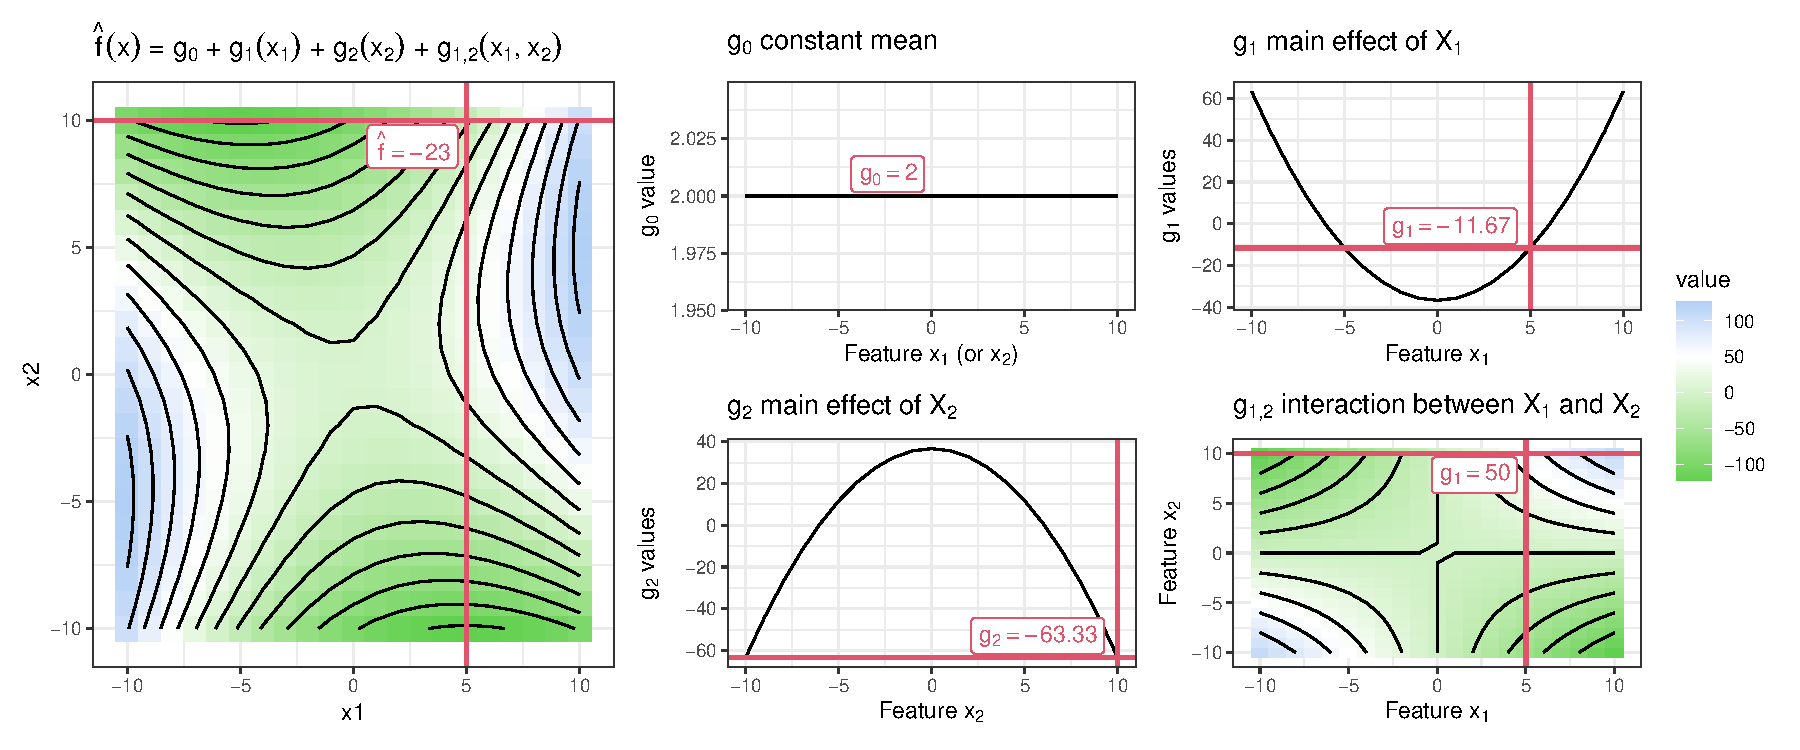
\includegraphics[width = \textwidth]{figure/decomposition}
    % \end{itemize}
    
    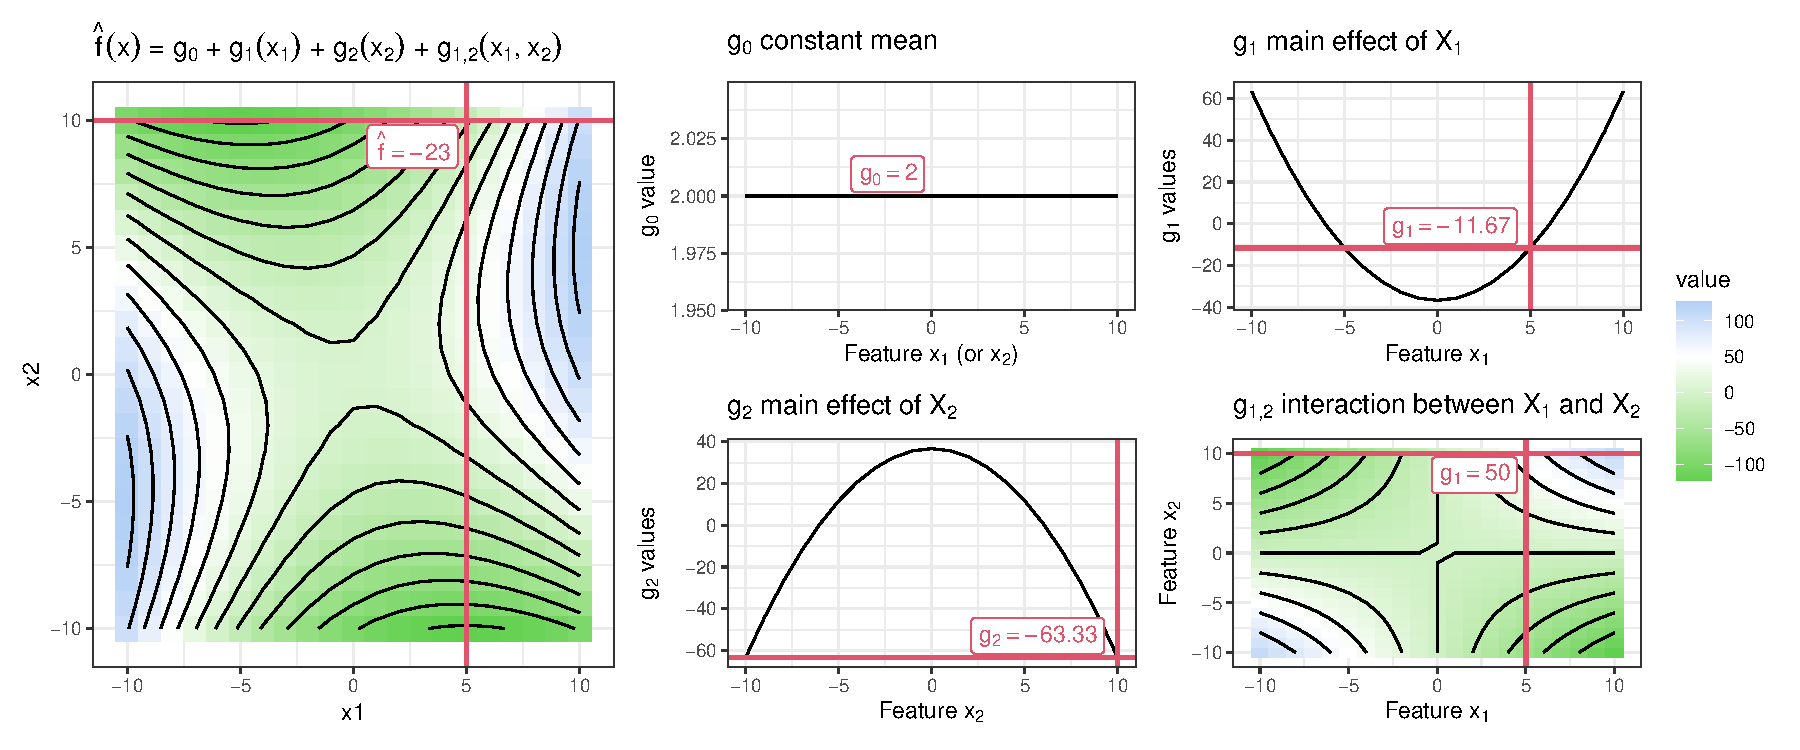
\includegraphics[width = \textwidth]{figure/decomposition}
    
    $\leadsto$ More details on this example later
        
    \end{example}
    
\end{frame}

\begin{frame}{Another example: Additive decomposition}

    \begin{example}

        % Consider the function

        $$
        \fh(x_1, x_2, x_3) = - 2x_1 - 2\sin(x_3) + |x_1|x_2 + 0.5 x_1 x_2 x_3 - \sin(x_2 x_3) + 1
        $$

        % We can again find the additive decomposition by reading from the functional formula, but some terms are empty, because certain types of effects and interactions are not present:
        Again, read additive decomposition from formula:
        \pause
        \begin{equation}\label{eq:func_decomp_second_min_example}
        \begin{aligned}
            & g_\emptyset(x_1, x_2, x_3) = 1 & \text{ constant part, no effects}  \\
            &
            \left.\begin{aligned}
                & g_1(x_1, x_2, x_3) = - 2x_1 \\
                & g_2(x_1, x_2, x_3) = 0 \\
                & g_3(x_1, x_2, x_3) = - 2\sin(x_3)
            \end{aligned}\right\}
                & \text{ main effects, no interactions}  \\
            &
            \left.\begin{aligned}
                & g_{1,2}(x_1, x_2, x_3) = |x_1|x_2 \\
                & g_{1,3}(x_1, x_2, x_3) = 0 \\
                & g_{2,3}(x_1, x_2, x_3) = - \sin(x_2 x_3)
            \end{aligned}\right\}
                & \text{ 2-way interactions (depending on 2 features)}  \\
            & g_{1,2,3}(x_1, x_2, x_3) = 0.5 x_1 x_2 x_3 & \text{ 3-way interactions}  \\
        \end{aligned}
        % \begin{matrix}
        %     g_\emptyset(x_1, x_2) = 4 &  \text{ Parts depending on no features at all (constant)}  \\
        %     g_1(x_1, x_2) = 2x_1 & \text{ Parts depending on a single feature (main effects)} \\
        %     g_1(x_1, x_2) =  0.3 e^{x_2} & \\
        %     g_{1,2}(x_1, x_2) = |x_1|x_2 & \text{ Part depending on both features (interaction)}  \\
        % \end{matrix}
        \end{equation}
        \(\Rightarrow\) 8 components in total, but some empty $\leadsto$ Certain interactions not present
        
    \end{example}
    
\end{frame}

\begin{frame}{General Form of Functional Decomposition
%\\
%% OLD
%\citebutton{Sobol (1993)}{http://www.andreasaltelli.eu/file/repository/sobol1993.pdf}
% new
\furtherreading{Sobol_1993}
% % OLD
%\citebutton{Sobol (2003)}{https://doi.org/10.1016/S0951-8320(02)00229-6}
% new
\furtherreading{Sobol_2003}
%% OLD
%\citebutton{Li et al. (2001)}{https://doi.org/10.1021/jp010450t}
% new
\furtherreading{Li_2001}
% OLD
%\citebutton{Li and Rabitz (2011)}{https://doi.org/10.1007/s10910-011-9898-0}
% new
\furtherreading{Rabitz_2011}
% OLD
%\citebutton{Chastaing et al. (2012)}{https://doi.org/10.1214/12-EJS749}
% new
\furtherreading{Chastaing_2012}
}

%\textbf{High-Dimensional Model Representation (HDMR):} 

\begin{definition}
% For interpretation purposes, one might be interested in decomposing a square-integrable function $\fh: \R^p \mapsto \R$ into sum of components of different dimensions w.r.t. inputs $x_1, \ldots, x_p$: %
\textit{Functional decomposition}: Additive decomposition of a function $\fh: \R^p \mapsto \R$ into a sum of components of different dimensions w.r.t. inputs $x_1, \ldots, x_p$: 
% \begin{equation}
% \begin{split}
% \fh(\xv) = 
% \displaystyle\sum_{S \subseteq \{1,\ldots,p\}} g_{S}(\xv_S) = \; & g_{\open \emptyset \close} + g_{\open 1 \close}(x_1) + g_{\open 2 \close}(x_2) + \dots + g_{\open p \close}(x_p) + \\
% & g_{\open 1, 2 \close}(x_1, x_2) + \dots + g_{\open p-1, p \close}(x_{p-1}, x_p) + \dots + \\
% & g_{\open 1, 2, 3 \close}(x_1, x_2, x_3) + \dots + \dots + g_{\open 1,\ldots,p \close}(x_1, \ldots, x_p)
% \end{split}
% \end{equation}
\begin{equation*}
\begin{split}
\fh(\xv)
\; = \; \; & \sum_{S \subseteq \{1,\ldots,p\}} g_{S}(\xv_S) \\
\; = \; \; & g_{\open \emptyset \close} +
g_{\open 1 \close}(x_1) + g_{\open 2 \close}(x_2) + \dots + g_{\open p \close}(x_p) + \\
& g_{\open 1, 2 \close}(x_1, x_2) + \dots + g_{\open p-1, p \close}(x_{p-1}, x_p) + \dots + \\
& g_{\open 1, 2, 3 \close}(x_1, x_2, x_3) + \dots +
g_{\open 1, 2, 3, 4 \close}(x_1, x_2, x_3, x_4) + \dots +
g_{\open 1,\ldots,p \close}(x_1, \ldots, x_p)
\end{split}    
\end{equation*}
$\leadsto$ one component for every possible combination $S$ of indices
\end{definition}
Sort terms according to degree of interaction:
\begin{itemize}
\item $g_{\open \emptyset \close} \hat = $ Constant mean (intercept) %$\mathbb{E}_X (\fh(\xv)) $
\item $g_{\open j \close} \hat = $ first-order or main effect of $j$-th feature alone on $\fh(\xv)$
\item $g_{\open j, k \close} \hat = $ second-order interaction effect of features $j$ and $k$ w.r.t. $\fh(\xv)$%, etc.
\item $g_{S}(\xv_S) \hat = $ $|S|$-order effect, depends \textbf{only} on features in $S$ %$x_j$ for all $j \in S$
\end{itemize}
\lz
\end{frame}

% TO DO: Put an example from a real-world dataset here for illustration purposes

\begin{frame}{Properties of the definition}
\begin{itemize}
    \item \textbf{Interpretability}: Extremely powerful decomposition, reveals complete interaction structure
    \pause
    \item Compare to GAM: Same decomposition, but without interactions \\
    $\implies$ Any GAM already comes with its decomposition
    $$
    \fh (\xv) = g_\emptyset + g_1(x_1) + g_2(x_2) + \ldots + g_p(x_p)
    $$
    \item Same for LMs: Decomposition explicitly modeled
    \pause
    \item Easy decomposition also for decision trees and tree ensembles (see below)
    \pause
    \item \textbf{Problem 1:} Calculating decomposition extremely difficult, often infeasible
    \begin{itemize}
        \item For \(p\) features: Decomposition with \(2^p\) terms \(\rightarrow\) too many different terms, difficult to interpret
    \end{itemize}
    \pause
    \item \textbf{Problem 2:} Definition not complete: Decomposition not unique, many trivial decompositions not useful
    \begin{itemize}
        \item[$\rightarrow$] More requirements or constraints needed to ensure decomposition is meaningful
        \item Even worse once features are dependent or correlated (see later)
    \end{itemize}
    % This 
    % Compare to GAM: The same decomposition is used, but in case of GAM, no interactions at all are considered, only main effects. I.p. any GAM already comes with its decomposition! \\
    % Same for linear models / linear regression and GLMs: The decomposition is explicitly modeled and directly follows from the model structure.

    % Somewhat similar for decision trees and tree ensembles (see below)
    % Super nice and extremely powerful decomposition! "Holy Gral of interpreting complex models"\\
    % BUT 2 Problems:
    % \begin{itemize}
    %     \item Definition not complete, such decomposition is not unique, and many trivial decompositions are not useful at all (see next slide) \\
    %         This problem get's much worse, whenever features are not independent \\
    %     \textbf{N.B.:} %Further constraints are required to obtain an unique and optimal solution for the components
    %     A unique solution for the components only exists under certain assumptions $\leadsto$ constraints, see later
        %and constraints
        %independent inputs and a \textit{vanishing condition}
        %$$\mathbb{E}_{X_j} (g_{S}(\xv_S)) = \int g_{S}(\xv_S) d \mathbb{P}(x_j) = 0, \forall j \in S, \forall S \subseteq \{1, \ldots, p\}$$
        %Without further constraints on components, there is no unique solution.
        %\end{itemize}
    %     \item Calculating such a decomposition is super, super hard in practice \\
    %         See for example: For \(p\) features, the decomposition has \(2^p\) terms \(\Rightarrow\) not very meaningful to interpret so many different terms \\
    % \end{itemize}
\end{itemize}
\end{frame}

\begin{frame}{Problem 2: Definition not enough}

    \begin{example}
        Again consider
        $$
        \fh(x_1, x_2, x_3) = - 2x_1 - 2\sin(x_3) + |x_1|x_2 + 0.5 x_1 x_2 x_3 - \sin(x_2 x_3) + 1
        $$
        \pause
        Two possible decompositions (valid according to definition):
        $$
            g_{1, \dots, p}(x_1, \dots, x_p) := \fh(\xv) \text{ and for all other terms } g_S(\xv_S) := 0 ,
        $$
        or:
        \begin{align*}
            g_\emptyset & = 1 \,;\quad
            g_1(x_1) = x_1 \,;\;
            g_2(x_2) = 2x_2 \,;\;
            g_3(x_3) = 3x_3 \,;\quad \\
            g_{1,2}(x_1, x_2) & = \frac{1}{2} x_1 x_2 \,;\;
            g_{1,3}(x_1, x_3) = \frac{1}{3} x_1 x_3 \,;\;
            g_{2,3}(x_2, x_3) = \frac{2}{3} x_2 x_3 \,;\; \\
            \text{ and} \quad
            & g_{1,2,3}(x_1, x_2, x_3) = \fh(x_1, x_2, x_3) - \sum_{S \subsetneqq \{1,2,3\}} g_S(\xv_S)
        \end{align*}
    \end{example}
    % Use $g_{1, \dots, p}(x_1, \dots, x_p) := \fh(\xv)$ and $g_S(\xv_S) := 0$ for all other terms
    \pause
    \(\implies\) Definition of decomposition not unique \\
    
\end{frame}

\begin{frame}{Example: Decision Trees}

\only<1,2>{
Define \textit{interaction type $t$} of a node: subset of features involved in constructing this node.

\textbf{Example:}

\begin{center}
    \begin{tikzpicture}[
    node/.style = {scale=1},
    scale = 1
    ]
        
        \node[node] at (0,2)(root){\(\R^d\)};
        
        \node[node] at (3,.5)(right_child){\(x_2 > 0\)};
        \node[node] at (4,-1)(rightright_grandchild){$x_3 > 1$};
        \node[node] at (2,-1)(rightleft_grandchild){\(x_3 \leq 1\)};
        
        \node[node] at (-3,.5)(left_child){\(x_2 \leq 0\)};
        \node[node] at (-4,-1)(leftleft_grandchild){$x_4 \leq -1$};
        \node[node] at (-1,-1)(leftright_grandchild){\(x_4 > -1\)};
        
        \node[node] at (-2,-2.5)(low_child_1){$x_1 \leq -0.5$};
        \node[node] at (-0,-2.5)(low_child_2){$x_1 > -0.5$};

        \draw[->, shorten >= 1pt, shorten <= 1pt] (root) -- (left_child);
        \draw[->, shorten >= 1pt, shorten <= 1pt] (root) -- (right_child);
        \draw[->, shorten >= 1pt, shorten <= 1pt] (left_child) -- (leftleft_grandchild);
        \draw[->, shorten >= 1pt, shorten <= 1pt] (left_child) -- (leftright_grandchild);
        \draw[->, shorten >= 1pt, shorten <= 1pt] (right_child) -- (rightright_grandchild);
        \draw[->, shorten >= 1pt, shorten <= 1pt] (right_child) -- (rightleft_grandchild);
        
        \draw[->, shorten >= 1pt, shorten <= 1pt] (leftright_grandchild) -- (low_child_1);
        \draw[->, shorten >= 1pt, shorten <= 1pt] (leftright_grandchild) -- (low_child_2);

        \only<2>{
        \node[node, color=red] at (0,1.5)(root_type){$t=\{\}$};
        
        \node[node, color=red] at (3,0)(right_child_type){$t=\{2\}$};
        \node[node, color=red] at (4,-1.5)(rightright_grandchild_type){$t=\{2,3\}$};
        \node[node, color=red] at (2,-1.5)(rightleft_grandchild_type){$t=\{2,3\}$};
        
        \node[node, color=red] at (-3,0)(left_child_type){$t=\{2\}$};
        \node[node, color=red] at (-4,-1.5)(leftleft_grandchild_type){$t=\{2,4\}$};
        \node[node, color=red] at (-1,-1.5)(leftright_grandchild_type){$t=\{2,4\}$};
        
        \node[node, color=red] at (-2,-3)(low_child_1_type){$t=\{1,2,4\}$};
        \node[node, color=red] at (0,-3)(low_child_2_type){$t=\{1,2,4\}$};
        
        }

    \end{tikzpicture}
\end{center}
}

\only<2>{
$\Rightarrow$ Degree of interaction in each node is \(|t|\).
}
    
\end{frame}

\begin{frame}{Decomposition for Decision Trees}
    
% [show that one decision tree directly comes with its functional decomposition using indicator functions]\\

Here: Decomposition via indicator functions
$$
\fh(\xv) = g_\emptyset + g_{2,4}(x_2, x_4) + g_{2,3}(x_2, x_3) + g_{1, 2, 4}(x_1, x_2, x_4)
$$
$\implies$ Decomposition has no main effect, but model certainly contains an effect of e.g. $x_2$

$\implies$ Lower-order effects ``hidden'' inside higher-order terms

$\leadsto$ reading from decision tree not enough, ``bad decomposition''

% \textbf{Problem again: uniqueness} If only reading from decision tree using indicator functions, lower-order effects may be hidden inside higher-order terms? \\

% Above example: Decomposition no main effect, but model certainly contains main effect of e.g. $x_2$.\\

\pause
\textbf{Note:} % OLD
%\citebutton{Yang (2024)}{https://arxiv.org/abs/2410.19098}
% new
\furtherreading{Yang_2024} propose a (quite complicated) solution for this case
% \(\Rightarrow\) Too complicated? Rather explain this in constraint-chapter or in other methods-chapter?

\end{frame}



\begin{frame}{Example: EBM}

    \begin{itemize}
        \item See before: \textbf{GAMs} have functional decomposition by definition
        \item \textbf{EBMs:} Sum of the final one- and two-dimensional components
        % \item \textbf{Similar: EBMs} Use the final one- and two-dimensional components % visualized in the end
        {
        \centering
        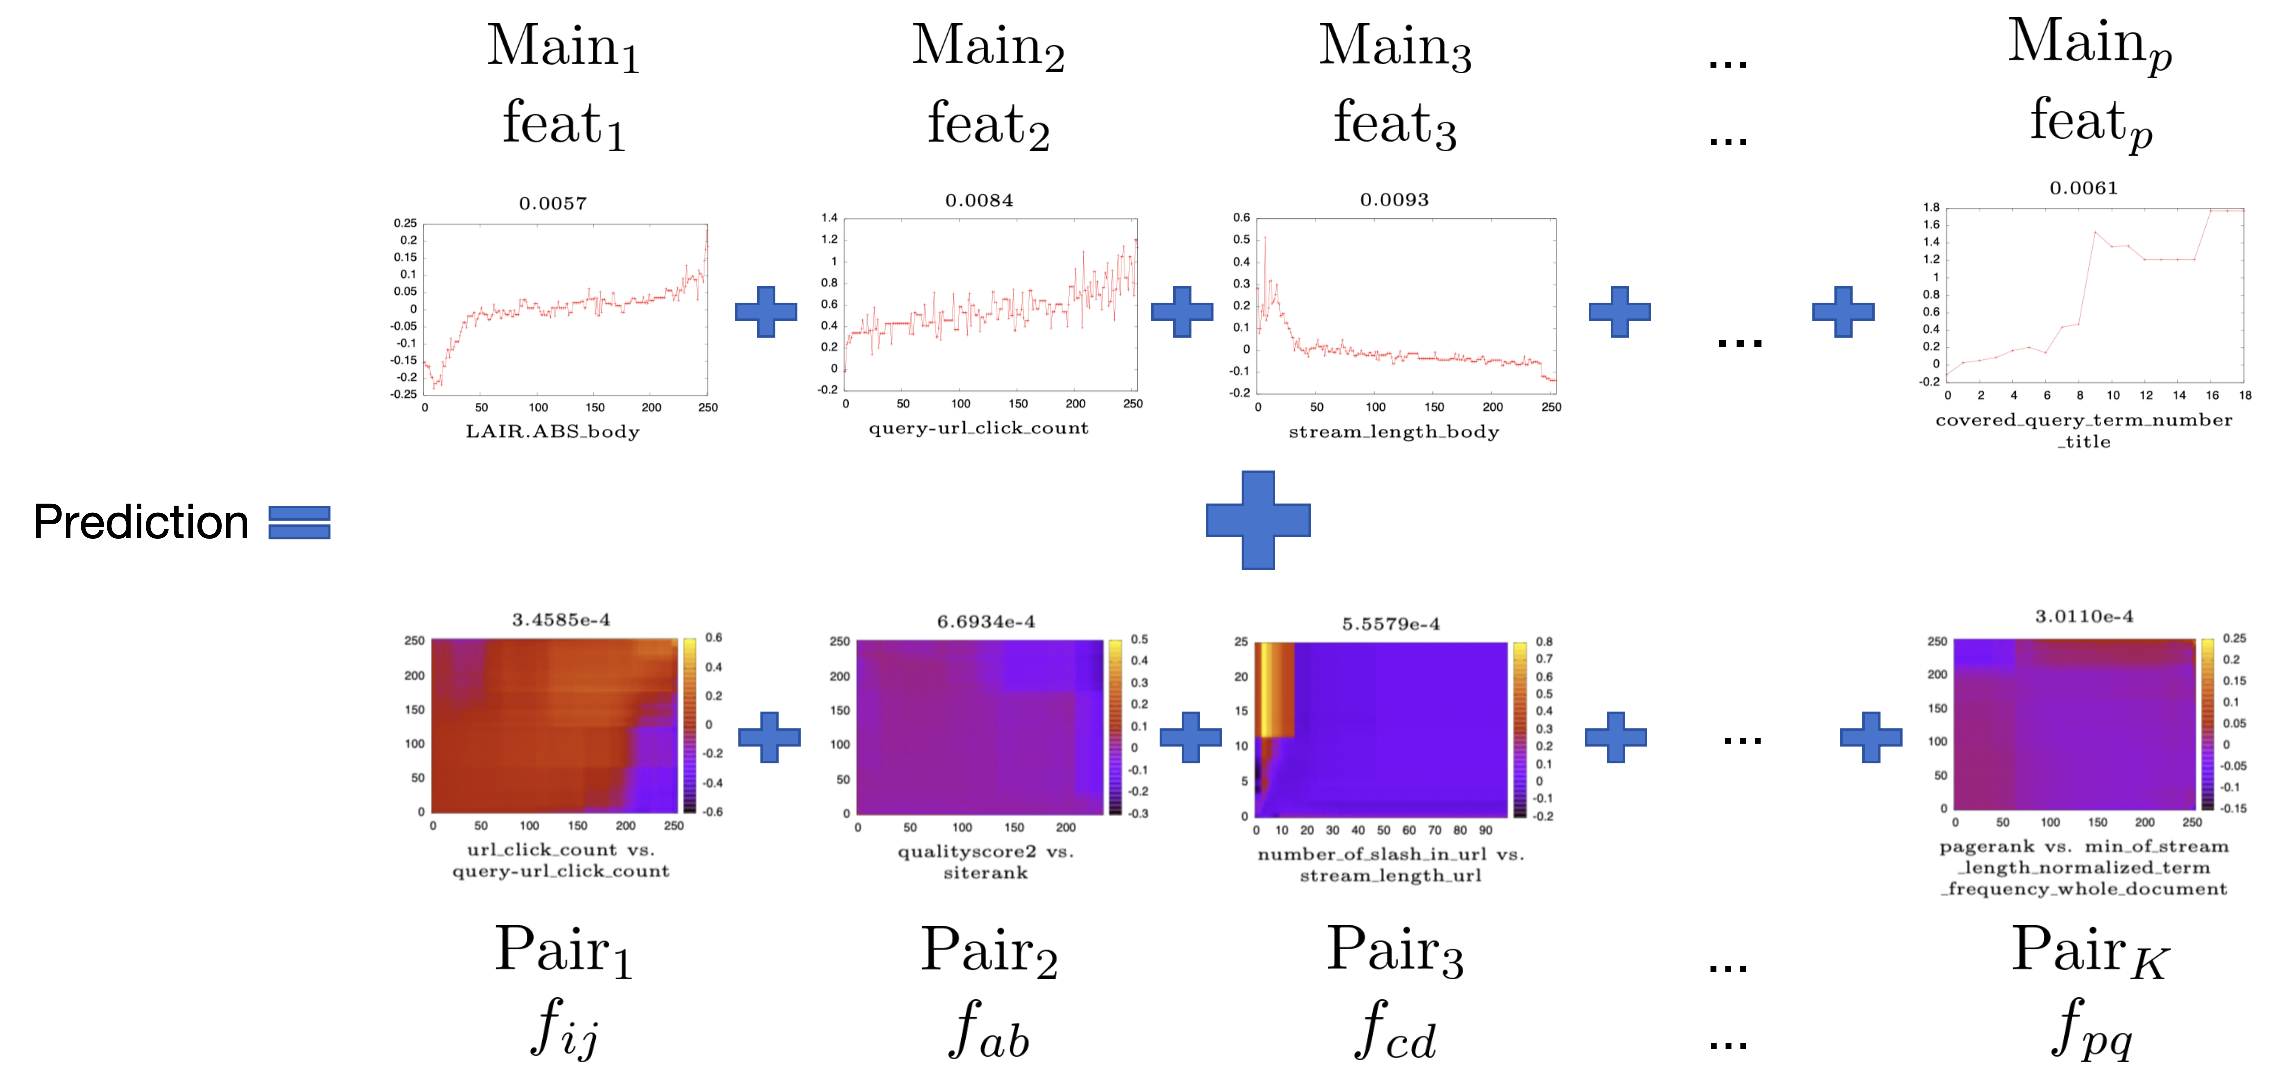
\includegraphics[width=\linewidth]{figure/final_ebm.png}
        }
        \only<2>{
        \item In general: Model with functional decomposition up to max. order 2 is always ``inherently interpretable''
        \item \textbf{Reason:} Visualization of all components
        } 
    \end{itemize}
    
\end{frame}

% \begin{frame}{High-dimensional modl representation (HDMR)}
%     [explain link to HDMR?? Or at end of chapter ?]

%     same for Sobol-Hoeffding decomposition
% \end{frame}

\endlecture
\end{document}
